\documentclass[12pt,a4paper]{article}

\usepackage[top=2.5cm,bottom=2.5cm,left=2.7cm,right=2.7cm]{geometry}
\usepackage[T1]{fontenc}
\usepackage[utf8]{inputenc}
\usepackage{lmodern}
\usepackage{microtype}
\usepackage{booktabs}
\usepackage{longtable}
\usepackage{array}
\usepackage{tabularx}
\usepackage{ragged2e}
\usepackage{multirow}
\usepackage{enumitem}
\usepackage{xcolor}
\usepackage{hyperref}
\usepackage{fancyhdr}
\usepackage{titlesec}
\usepackage{parskip}
\usepackage{amssymb}
\usepackage{float}
\usepackage{colortbl}
\usepackage{graphicx}
\usepackage{tikz}
\usetikzlibrary{positioning, shapes.geometric, arrows.meta, fit, backgrounds, calc}

\definecolor{headerblue}{RGB}{20,62,128}
\definecolor{textgray}{RGB}{75,75,75}
\definecolor{accent}{RGB}{32,113,167}
\definecolor{rowlight}{RGB}{237,244,252}
\definecolor{rowwhite}{RGB}{255,255,255}
\definecolor{tableheader}{RGB}{20,62,128}
\definecolor{tablerule}{RGB}{160,185,215}
\definecolor{modcms}{RGB}{52,152,219}
\definecolor{modscholar}{RGB}{46,204,113}
\definecolor{modevents}{RGB}{231,76,60}
\definecolor{modvenue}{RGB}{155,89,182}
\definecolor{modsystem}{RGB}{241,196,15}

% Enhanced table styling
\renewcommand{\arraystretch}{1.35}
\arrayrulecolor{tablerule}

\hypersetup{
  colorlinks=true,
  linkcolor=headerblue,
  urlcolor=accent,
  pdftitle={Software Requirements Specification - Digital Department Hub},
  pdfauthor={du\_vagabond}
}

\pagestyle{fancy}
\fancyhf{}
\lhead{\small\color{textgray}SRS v1.1 | Digital Department Hub}
\rhead{\small\color{textgray}CMS, Events, Scholarships, and Resource Booking}
\cfoot{\thepage}
\renewcommand{\headrulewidth}{0.4pt}
\setlength{\headheight}{14.5pt}

\titleformat{\section}
  {\large\bfseries\color{headerblue}}
  {\thesection}{0.75em}{}[\vspace{-4pt}\rule{\linewidth}{0.5pt}]
\titleformat{\subsection}
  {\normalsize\bfseries\color{textgray}}
  {\thesubsection}{0.6em}{}

\newcolumntype{L}[1]{>{\RaggedRight\arraybackslash}p{#1}}
\newcolumntype{C}[1]{>{\Centering\arraybackslash}p{#1}}
\newcolumntype{Y}{>{\RaggedRight\arraybackslash}X}

% Styled table header command
\newcommand{\thead}[1]{\textbf{\color{white}#1}}
\newcommand{\theadrow}{\rowcolor{headerblue}}

% Allow LaTeX to break long camelCase entity names
\hyphenation{Scholar-ship-Category Scholar-ship-Notice Scholar-ship-Application Scholar-ship-Update Recipient-Publication Event-Registration Event-Feedback Venue-Booking Contact-Inquiry Gallery-Album Media-Item News-Post Audit-Log}

\begin{document}

\pagenumbering{gobble}

\begin{titlepage}
\centering
\vspace*{0.3cm}

% University logo placeholder
\IfFileExists{logo.png}{%
  
\includegraphics[width=2.8cm]{logo.png}%
}{%
  \fbox{\begin{minipage}[c][2.8cm][c]{2.8cm}\centering\textbf{Logo}\\\texttt{logo.png}\end{minipage}}%
}
\par\vspace{0.2cm}
{\Large\bfseries University of Dhaka\par}
\vspace{0.15cm}
{\large Department of Computer Science and Engineering\par}

\vspace{0.6cm}
{\Huge\bfseries\color{headerblue}Software Requirements Specification\par}
\vspace{0.3cm}
{\LARGE\bfseries Digital Department Hub\par}
\vspace{0.15cm}
{\large CMS, Events, Scholarships, and Resource Booking\par}
\vspace{0.5cm}
\rule{0.82\textwidth}{1pt}\par
\vspace{0.35cm}
{\renewcommand{\arraystretch}{1.15}%
\begin{tabular}{@{}ll@{}}
\textbf{Course:} & CSE-4113 Internet Programming Lab \\
\textbf{Document Type:} & Software Requirements Specification (SRS) \\
\textbf{Version:} & 1.1 \\
% \textbf{Status:} & Draft for Lab 2 Submission \\
\textbf{Date:} & April 10, 2026 \\
% \textbf{Project Code:} & Project A \\
\textbf{Document ID:} & SRS-PA-2026-01 \\
\textbf{Prepared By:} & du\_vagabond \\
\end{tabular}}
\vspace{0.35cm}
\par\rule{0.82\textwidth}{1pt}

\vspace{0.4cm}
{\large\textbf{Submitted to:}\par}
\vspace{0.15cm}
\begin{tabular}{@{}l@{}}
Prof.\ Dr.\ Md.\ Mamun Or Rashid \\
Mr.\ Md.\ Fahim Arefin \\
Mr.\ Md.\ Ahasanul Alam \\
\end{tabular}

\vfill
{\large Submitted for Lab 3:  SRS v1.1\par}
\end{titlepage}

\clearpage
\pagenumbering{roman}
\tableofcontents
\newpage
\pagenumbering{arabic}

\section{Document Control}

\subsection{Metadata}

\rowcolors{2}{rowlight}{rowwhite}
\begin{tabularx}{\textwidth}{@{}l Y@{}}
\theadrow \thead{Field} & \thead{Value} \\
Project Name & Digital Department Hub: CMS, Events, Scholarships, and Resource Booking \\
Project Scope & Dynamic website, CMS, scholarship management, event management, venue booking \\
Course & CSE-4113 Internet Programming Lab \\
Document Version & 1.1 \\
Document Status & Draft \\
Date & April 10, 2026 \\
Prepared For & Lab 3 Submission \\
Repository URL & https://github.com/Ovijit-Balo/Digital-Department-Hub.git \\
\end{tabularx}
\rowcolors{0}{}{}

\subsection{Authors and Reviewers}

\rowcolors{2}{rowlight}{rowwhite}
\begin{tabularx}{\textwidth}{@{}l l Y l@{}}
\theadrow \thead{Role} & \thead{Name} & \thead{Email} & \thead{Date} \\
Author & Showkoth Osman Shova & showkoth-2021711187@cs.du.ac.bd & March 8, 2026 \\
Author & Ovijit Chandra Balo & ovijit-2021711204@cs.du.ac.bd & March 8, 2026 \\
Author & Shraban Karmoker Avi & shrabankarmoker-2021911220@cs.du.ac.bd & March 8, 2026 \\
Author & Md. Khairul Mia &  mdkhairulmia145@gmail.com & March 8, 2026 \\
\end{tabularx}
\rowcolors{0}{}{}

\subsection{Revision History}

\rowcolors{2}{rowlight}{rowwhite}
\begin{tabularx}{\textwidth}{@{}l l l Y@{}}
\theadrow \thead{Version} & \thead{Date} & \thead{Author} & \thead{Change Description} \\
0.1 & March 7, 2026 & du\_vagabond & Initial project-specific draft prepared from lab template \\
1.0 & March 8, 2026 & du\_vagabond & Detailed SRS completed for Lab 2 submission \\
1.1 & April 10, 2026 & du\_vagabond & Clarified ambiguous requirements, added notification and applicant tracking workflows, and refined measurable NFR targets \\
\end{tabularx}
\rowcolors{0}{}{}

\newpage
\section{Problem Definition}

\subsection{Problem Statement}

Many academic departments still manage their public websites, announcements, scholarship notices, and event logistics using disconnected tools such as static pages, spreadsheets, social media posts, email threads, and manual office communication. This creates several operational and communication failures.

First, website content becomes outdated because non-technical administrative staff cannot independently edit pages, publish notices, or update departmental information. As a result, students, guardians, alumni, donors, and external partners often see incomplete or obsolete information.

Second, scholarship-related activities are difficult to manage transparently. Notices may be shared inconsistently, application windows may not be tracked properly, applications are often reviewed manually through paper or spreadsheet-based processes, and recipient publication may be delayed. This reduces fairness, traceability, and administrative efficiency.

Third, department events, auditorium reservations, and lab bookings are frequently handled by phone calls, informal requests, or ad hoc spreadsheets. This creates booking conflicts, weak approval tracking, low visibility of available venues, and poor attendee management. In addition, there is no structured mechanism for event registration, attendance verification, or feedback collection.

This project addresses these problems by proposing a unified departmental platform that combines a public-facing bilingual website, an administrative content management system, scholarship management, public engagement tools, event publication and registration, and a controlled venue reservation workflow.

\subsection{Why the Problem Matters}

The department's digital presence directly influences public perception, student engagement, and administrative responsiveness. A reliable website improves communication quality and institutional credibility. A structured scholarship system improves fairness, accountability, and student access to opportunities. A centralized event and booking system improves operational coordination, reduces double-booking, and supports better planning for classes, seminars, workshops, and public programs.

\subsection{Target Users}

\rowcolors{2}{rowlight}{rowwhite}
\begin{longtable}{@{}L{3.6cm}L{5.2cm}L{5cm}@{}}
\theadrow \thead{User Group} & \thead{Description} & \thead{Main Needs} \\
\endhead
Public Visitors & Prospective students, parents, alumni, employers, donors, and external visitors & Browse departmental information, news, events, gallery items, and announcements \\
Current Students & Enrolled students who interact frequently with scholarship and event modules & View notices, apply for scholarships, register for events, see booking-related updates \\
Administrative Staff & Non-technical staff responsible for routine content publishing and inquiry handling & Update pages, news, notices, and public information without programming knowledge \\
Faculty Members & Teachers or coordinators who may publish content or request venue bookings & Submit bookings, manage event details, review public communication \\
Scholarship Committee & Faculty or staff responsible for scholarship review and publication & Publish notices, review applications, export data, publish recipient lists \\
Event Managers & Organizers managing seminars, workshops, competitions, and outreach events & Publish events, manage registrations, check in participants, collect feedback \\
Venue Administrators & Staff overseeing auditorium, lab, and room reservations & View requests, approve or reject bookings, monitor schedule conflicts \\
System Administrators & Technical or authorized supervisors with full control of the platform & Manage users, roles, settings, configurations, and audit oversight \\
\bottomrule
\end{longtable}
\rowcolors{0}{}{}

\subsection{Goals and Non-Goals}

\textbf{Goals}
\begin{itemize}[nosep]
\item Provide a professional public-facing departmental website with dynamic content.
\item Enable non-technical staff to manage pages, blogs, notices, and media using a WYSIWYG CMS.
\item Support Bangla and English content for public communication.
\item Centralize scholarship notice publication, application intake, review, export, and recipient publication.
\item Support event publication, calendar display, registration, QR-based check-in, and feedback.
\item Provide a reservation workflow for auditorium, lab, and selected rooms.
\item Improve transparency, reduce manual work, and prevent scheduling conflicts.
\end{itemize}

\textbf{Non-Goals}
\begin{itemize}[nosep]
\item No online payment gateway for event fees or scholarship disbursement in the first release.
\item No integration with the university ERP, finance system, or central student information system in the first release.
\item No native Android or iOS application; the platform will be web-based and responsive.
\item No automatic machine translation beyond manual translation workflow support.
\item No multi-department, multi-campus, or multi-tenant architecture in the initial scope.
\end{itemize}

\section{Scope and Context}

\subsection{In Scope}

\begin{itemize}[nosep]
\item Public website pages such as home, about, faculty, announcements, news, blog, gallery, scholarships, events, contact, and booking-related information.
\item CMS administration panel for page creation, editing, publishing, translation, media management, and SEO metadata.
\item News, blog, and announcement management with categories, tags, images, and publication control.
\item Bangla/English language switching with field-level translation support.
\item Media gallery with support for image and video content.
\item Contact and inquiry form with admin-side response tracking.
\item Scholarship management including notice publication, application windows, category definitions, review process, export, and recipient list publishing.
\item Event publication, event calendar, registration workflow, QR-based attendance verification, and feedback collection.
\item Auditorium, lab, and room booking with conflict detection and approval workflow.
\item Role-based administrative access control across different modules.
\end{itemize}

\subsection{Out of Scope}

\begin{itemize}[nosep]
\item Automatic scholarship payment or banking integration.
\item University-wide single sign-on and centralized identity federation.
\item Learning management system integration.
\item Advanced business analytics beyond operational reporting required by the modules.
\item Dedicated mobile apps.
\item External social media campaign management beyond metadata support for sharing.
\end{itemize}

\subsection{Assumptions and Constraints}

\textbf{Technical Constraints}
\begin{itemize}[nosep]
\item The system will run as a web application over standard modern browsers.
\item The platform must store and render Unicode content correctly for Bangla and English.
\item All admin and public form interactions require a stable server-side database.
\item Public users should not be required to install any application for QR check-in participation.
\end{itemize}

\textbf{Organizational Constraints}
\begin{itemize}[nosep]
\item Non-technical staff must be able to publish content with minimal training.
\item Scholarship applicant data may contain personally identifiable information and must be protected accordingly.
\item Booking approval must remain under manual administrative control.
\end{itemize}

\textbf{Timeline Constraints}
\begin{itemize}[nosep]
\item This document is prepared for Lab 2 submission.
\item The first implementation milestone is expected to prioritize the public website and CMS.
\item Scholarship and event/booking modules may be delivered incrementally after the core website foundation.
\end{itemize}

\section{Stakeholders and Roles}

\subsection{Stakeholders}

\rowcolors{2}{rowlight}{rowwhite}
\begin{longtable}{@{}L{4cm}L{7cm}C{2cm}@{}}
\theadrow \thead{Stakeholder} & \thead{Interest} & \thead{Priority} \\
\endhead
Department Head & Better public communication, institutional branding, and operational visibility & High \\
Administrative Office & Efficient daily content and inquiry management & High \\
Students & Easy access to news, scholarships, and event participation & High \\
Scholarship Committee & Transparent, trackable scholarship administration & High \\
Faculty Members & Reliable event and venue coordination & Medium \\
Event Organizers & Simplified publishing, registration, and attendance management & Medium \\
IT Support Team & Secure, maintainable, and manageable system operation & High \\
Public Visitors & Reliable and current department information & Medium \\
\bottomrule
\end{longtable}
\rowcolors{0}{}{}

\subsection{User Roles and Permissions}

\rowcolors{2}{rowlight}{rowwhite}
\begin{longtable}{@{}L{3.4cm}L{4.4cm}L{6.3cm}@{}}
\theadrow \thead{Role} & \thead{Description} & \thead{Permissions} \\
\endhead
Super Admin & Highest-level administrator & Manage users, roles, system settings, content, scholarship, events, booking, and audit visibility \\
Content Editor & Staff responsible for public information management & Create, edit, review, publish pages, news, blogs, galleries, translations, and SEO metadata \\
Scholarship Manager & Authorized scholarship operator & Create categories, publish notices, open/close applications, review submissions, export data, publish recipients \\
Event Manager & Organizer of departmental events & Create and publish events, manage registrations, generate QR codes, view check-in and feedback \\
Venue Administrator & Controller of venue schedules & Review booking requests, approve/reject bookings, block unavailable slots, monitor conflicts \\
Applicant & Student or other eligible person applying for scholarship & View notices, submit applications, track own status if login/tracking is enabled \\
Event Registrant & Public or student participant & Register for event, receive QR confirmation, submit post-event feedback \\
Public Visitor & Read-only visitor & Browse public content and submit contact forms \\
\bottomrule
\end{longtable}
\rowcolors{0}{}{}

\section{Functional Requirements}

Requirement identifiers follow the format \texttt{FR-PA-\#\#\#}. Priority values: \textbf{M} = Must, \textbf{S} = Should, \textbf{C} = Could.

\rowcolors{2}{rowlight}{rowwhite}
\begin{longtable}{@{}L{2cm}L{2.4cm}L{6cm}C{0.9cm}L{3.4cm}@{}}
\theadrow \thead{Req ID} & \thead{Feature} & \thead{Requirement Statement} & \thead{Pri.} & \thead{Acceptance Criteria} \\
\endhead

\rowcolor{modcms!15}\multicolumn{5}{@{}l}{\textit{\textbf{\color{modcms}CMS and Website Management}}}\\
FR-PA-001 & CMS & The system shall allow authorized editors to create, edit, preview, and publish dynamic web pages using a WYSIWYG interface. & M & Editor can create a page without writing HTML; preview and published view are consistent. \\
FR-PA-002 & CMS & The system shall support content states of draft, under review, and published for pages, news, blogs, and notices. & M & Unpublished items are not visible publicly; state transitions are stored correctly. \\
FR-PA-003 & CMS & The system shall support reusable page templates for homepage, standard content page, and campaign/landing page. & S & Editor can select template during creation and published page matches selected layout. \\
FR-PA-004 & CMS & The system shall maintain version history for edited content and allow rollback to a prior revision. & S & At least one previous version can be restored successfully. \\
FR-PA-005 & Navigation & The system shall allow administrators to manage top-level navigation menus and footer links from the CMS. & M & Menu changes appear on the public site after save/publish. \\
FR-PA-006 & Localization & The system shall store Bangla and English values for all translatable public fields, including at minimum page title, page body, news/blog title, news/blog body, event title, event description, scholarship notice title, and scholarship notice description. & M & Users can view the same content item in either language when translations exist; listed fields are available in both language variants in admin forms. \\
FR-PA-007 & Localization & The system shall indicate untranslated fields to content editors. & S & Missing translation fields are visually flagged in the admin panel. \\
FR-PA-008 & Localization & The system shall provide a visible public language switcher on all major public pages. & M & Visitor can change language from any main public page. \\
FR-PA-009 & News/Blog & The system shall allow editors to create news and blog posts with title, body, category, tags, cover image, and publish date. & M & New posts appear on public listing pages after publication. \\
FR-PA-010 & News/Blog & The system shall support scheduled publishing of news and blog posts. & S & Post remains hidden before schedule time and becomes visible automatically afterward. \\
FR-PA-011 & Gallery & The system shall allow image and video upload to categorized galleries or albums. & M & Uploaded media is retrievable by album and displayable on the public site. \\
FR-PA-012 & Gallery & The system shall generate display thumbnails for uploaded images. & M & Thumbnail appears in the gallery management interface after upload. \\
FR-PA-013 & Contact & The system shall provide a public contact/inquiry form with fields for name, email, subject, and message. & M & Valid inquiry creates a record and sends notification to admin. \\
FR-PA-014 & Contact & The system shall allow administrators to mark inquiries as new, in progress, or resolved. & S & Inquiry state changes are stored and visible in inquiry management view. \\
FR-PA-015 & SEO & The system shall allow entry of SEO metadata including title, description, keywords, canonical URL, and social sharing tags. & M & Metadata appears in generated HTML head section. \\
FR-PA-016 & SEO & The system shall generate and update an XML sitemap for published public pages. & M & Sitemap includes newly published public content URLs. \\

\rowcolor{modscholar!15}\multicolumn{5}{@{}l}{\textit{\textbf{\color{modscholar!80!black}Scholarship Management}}}\\
FR-PA-017 & Scholarship & The system shall allow scholarship managers to define multiple scholarship categories with different amounts and types. & M & Categories can be saved, edited, and selected during notice creation. \\
FR-PA-018 & Scholarship & The system shall support both one-off and monthly scholarships. & M & Notice and category forms store scholarship type and display it correctly on the public site. \\
FR-PA-019 & Scholarship & The system shall allow managers to publish scholarship notices with title, category, description, eligibility, amount, opening date, and deadline. & M & Published notice is visible on scholarship listing page with configured data. \\
FR-PA-020 & Scholarship & The system shall allow managers to independently open and close application windows for each scholarship notice. & M & System blocks new applications outside the configured open period. \\
FR-PA-021 & Scholarship & The system shall provide an online scholarship application form with configurable or predefined applicant fields. & M & Valid application is stored with status Pending. \\
FR-PA-022 & Scholarship & The system shall support attachment or document submission for scholarship applications if required by the committee. & S & Uploaded documents are linked to the correct application and retrievable for review. \\
FR-PA-023 & Scholarship & The system shall prevent duplicate applications to the same scholarship notice by the same applicant identity or email. & M & Repeated submission attempt is rejected with a clear message. \\
FR-PA-024 & Scholarship & The system shall allow managers to review applications and update their status as Pending, Shortlisted, Awarded, or Rejected. & M & Status changes persist and are visible in filtered lists. \\
FR-PA-025 & Scholarship & The system shall allow export of scholarship applications in CSV format for further analysis. & M & Exported row count matches application list count. \\
FR-PA-026 & Scholarship & The system shall allow export of scholarship applications in printable PDF report format. & S & PDF report includes core applicant and status information. \\
FR-PA-027 & Scholarship & The system shall allow publication of scholarship recipient lists after review completion. & M & Public recipient list includes only awarded applicants. \\
FR-PA-028 & Scholarship & The system shall allow posting updates related to a scholarship notice after its publication. & S & Updates appear in chronological order on the scholarship detail page. \\

\rowcolor{modevents!15}\multicolumn{5}{@{}l}{\textit{\textbf{\color{modevents!80!black}Events, Registration, and Check-In}}}\\
FR-PA-029 & Events & The system shall allow event managers to create events with bilingual title, description, venue, schedule, category, capacity, and registration deadline. & M & Published event appears on event listing and public calendar. \\
FR-PA-030 & Events & The system shall provide both list-based and calendar-based public event views. & M & Visitor can browse upcoming events from either view. \\
FR-PA-031 & Events & The system shall allow visitors or students to register for events using a registration form. & M & Successful registration creates a participant record. \\
FR-PA-032 & Events & The system shall enforce capacity limits and stop further registration after the event is full. & M & Additional users cannot register once maximum capacity is reached. \\
FR-PA-033 & Events & The system shall generate a unique QR code for each confirmed event registration. & M & Each registration has one unique QR code usable during check-in. \\
FR-PA-034 & Events & The system shall provide a QR-based check-in interface for authorized staff. & M & Staff can scan valid QR codes and mark attendance. \\
FR-PA-035 & Events & The system shall prevent double check-in of the same registration. & M & Second scan displays duplicate warning rather than creating another attendance entry. \\
FR-PA-036 & Events & The system shall support post-event feedback collection from registered or checked-in attendees. & S & Feedback form responses are saved and viewable in aggregate. \\
FR-PA-037 & Events & The system shall allow event managers to view registration counts, attendance counts, and feedback summaries. & S & Dashboard displays counts for a selected event. \\

\rowcolor{modvenue!15}\multicolumn{5}{@{}l}{\textit{\textbf{\color{modvenue!80!black}Venue Reservation and Booking}}}\\
FR-PA-038 & Booking & The system shall maintain a list of bookable venues including auditorium, labs, and optionally classrooms. & M & Authorized admin can add and edit venue records. \\
FR-PA-039 & Booking & The system shall allow authorized users to submit venue booking requests with venue, date, time, purpose, and expected attendance. & M & Request is stored with Pending status and visible to venue admin. \\
FR-PA-040 & Booking & The system shall automatically block creation of a booking request when the requested time overlaps an existing Approved or Blocked slot for the same venue. & M & Overlapping request cannot be submitted; system shows a conflict message identifying the unavailable interval. \\
FR-PA-041 & Booking & The system shall provide venue administrators with approve and reject actions and an optional comment field. & M & Approval decision updates booking status and stores comment. \\
FR-PA-042 & Booking & The system shall display an availability calendar for each venue. & M & Approved reservations appear in the correct calendar slots. \\
FR-PA-043 & Booking & The system shall allow administrators to block venue times for maintenance or institutional use. & S & Blocked slots cannot be requested by regular users. \\
FR-PA-044 & Booking & The system shall notify requesters about booking approval or rejection. & S & Requester receives visible status update and configured notification. \\

\rowcolor{modsystem!15}\multicolumn{5}{@{}l}{\textit{\textbf{\color{headerblue}Security, Accounts, and Administration}}}\\
FR-PA-045 & Auth & The system shall require authenticated access for all administrative functions. & M & Unauthenticated user cannot open protected admin routes. \\
FR-PA-046 & RBAC & The system shall implement role-based access control across CMS, scholarship, event, and booking modules. & M & Users can only access features permitted for their assigned role. \\
FR-PA-047 & Auth & The system shall support password reset for administrative users. & M & Valid reset request issues a time-limited reset workflow. \\
FR-PA-048 & Audit & The system shall record important administrative actions such as publish, status change, approval, and rejection events. & S & Action log shows actor, action type, target, and timestamp. \\
FR-PA-049 & Notifications & The system shall provide a unified notification service for key workflow events, including contact inquiry receipt, scholarship application submission, scholarship status change, event registration confirmation, event reminder, and booking decision. & M & For each configured trigger, the system creates an in-app notification log entry and sends email when email channel is enabled. \\
FR-PA-050 & Applicant Portal & The system shall provide applicant account login and a personal dashboard to track scholarship applications and statuses. & S & Applicant can sign in, view own application history, and see current status timeline per application. \\
FR-PA-051 & Applicant Portal & The system shall allow applicants to view submission details and uploaded document list for their own applications without exposing other applicants' data. & M & Authenticated applicant can open only own records; direct access to another applicant record is denied. \\
\bottomrule
\end{longtable}
\rowcolors{0}{}{}

\section{User Stories and Use Cases}

\subsection{User Stories}

\rowcolors{2}{rowlight}{rowwhite}
\begin{longtable}{@{}L{1.9cm}L{2.5cm}L{3.4cm}L{3.7cm}L{3.2cm}@{}}
\theadrow \thead{Story ID} & \thead{As a} & \thead{I want} & \thead{So that} & \thead{Acceptance Criteria} \\
\endhead
US-PA-001 & Content Editor & to edit website pages using a visual editor & I can maintain the site without coding knowledge & Page can be saved, previewed, and published successfully. \\
US-PA-002 & Content Editor & to provide both Bangla and English content & visitors can read in their preferred language & Language switcher displays the correct translation. \\
US-PA-003 & Public Visitor & to read updated news and announcements & I can stay informed about department activities & Published posts appear in reverse chronological order. \\
US-PA-004 & Scholarship Manager & to publish scholarship notices with opening and closing dates & applicants can apply within a controlled period & Apply option is only visible during active window. \\
US-PA-005 & Applicant & to apply for a scholarship online & I do not need manual paperwork or office visits & Valid application is submitted and confirmation is shown or sent. \\
US-PA-006 & Scholarship Manager & to review and filter applications by status & I can manage the selection process efficiently & Manager can search and update application statuses. \\
US-PA-007 & Scholarship Manager & to export applications & I can review them outside the system or share them with the committee & CSV/PDF export downloads correctly. \\
US-PA-008 & Event Manager & to publish an event with a registration form & participants can register online & Event appears publicly and registration accepts valid submissions. \\
US-PA-009 & Event Registrant & to receive a QR pass after registration & I can use it for faster check-in at the event & QR code is generated and linked to my registration. \\
US-PA-010 & Event Staff & to scan QR codes during check-in & I can confirm attendance quickly and accurately & Valid code marks attendee as checked in exactly once. \\
US-PA-011 & Venue Requester & to request the auditorium or a lab online & I can reserve spaces in a formal and trackable way & Request is stored and conflict-checked. \\
US-PA-012 & Venue Administrator & to approve or reject booking requests & I can manage space usage and avoid conflicts & Decision is recorded and communicated to requester. \\
US-PA-013 & Public Visitor & to browse image and video galleries & I can see departmental activities and achievements & Public gallery loads categorized media correctly. \\
US-PA-014 & Admin Staff & to track contact form submissions & I can respond to public inquiries systematically & Inquiry list shows status and messages. \\
US-PA-015 & Super Admin & to manage user roles & I can enforce secure access control & Created users can only access assigned modules. \\
US-PA-016 & Applicant & to log in and track my scholarship applications & I can follow progress without contacting the office repeatedly & Dashboard shows status and timeline for each submitted application. \\
US-PA-017 & System Administrator & to configure notification triggers and channels & stakeholders receive timely workflow updates & Triggered events create notification logs and optional emails as configured. \\
\bottomrule
\end{longtable}
\rowcolors{0}{}{}

\subsection{Critical Use Cases}

\subsubsection*{UC-PA-01: Submit Scholarship Application}

\textbf{Preconditions}
\begin{itemize}[nosep]
\item A scholarship notice has already been published.
\item The application window for that notice is currently open.
\item The applicant has access to the internet and the required information/documents.
\end{itemize}

\textbf{Main Flow}
\begin{enumerate}[nosep]
\item The applicant opens the scholarship listing page.
\item The applicant selects an active scholarship notice.
\item The system displays notice details and an application option.
\item The applicant completes the online form and uploads required documents if applicable.
\item The applicant submits the application.
\item The system validates all fields and stores the record with Pending status.
\item The system shows a success confirmation and may send an acknowledgment notification.
\end{enumerate}

\textbf{Alternate / Exception Flow}
\begin{itemize}[nosep]
\item If the application window is closed, the apply action is not available.
\item If required data is missing, the system rejects submission and highlights the errors.
\item If the same applicant attempts duplicate submission, the system blocks the request.
\end{itemize}

\textbf{Postconditions}
The application exists in the database and is available for scholarship manager review.

\subsubsection*{UC-PA-02: Register for Event and Check In Using QR Code}

\textbf{Preconditions}
\begin{itemize}[nosep]
\item An event has been published and registration is still open.
\item The event has not reached its maximum capacity.
\end{itemize}

\textbf{Main Flow}
\begin{enumerate}[nosep]
\item The visitor opens the event details page.
\item The visitor submits the registration form.
\item The system validates the form and creates a registration record.
\item The system generates a unique QR code for the registrant.
\item During the event, authorized staff opens the check-in interface.
\item Staff scans the attendee's QR code.
\item The system validates the token and marks the attendee as checked in.
\end{enumerate}

\textbf{Alternate / Exception Flow}
\begin{itemize}[nosep]
\item If capacity is full, the system blocks new registrations.
\item If the QR code is invalid, the system shows an error.
\item If the registrant was already checked in, the system shows a duplicate warning.
\end{itemize}

\textbf{Postconditions}
Attendance is recorded and available in event reporting.

\subsubsection*{UC-PA-03: Submit and Approve Venue Booking Request}

\textbf{Preconditions}
\begin{itemize}[nosep]
\item The requester is authorized to create booking requests.
\item The target venue is already configured in the system.
\end{itemize}

\textbf{Main Flow}
\begin{enumerate}[nosep]
\item The requester opens the booking calendar.
\item The requester selects a venue, date, and time range.
\item The requester enters purpose and attendance estimate.
\item The system checks existing approved bookings and blocked slots.
\item If no conflict is found, the system stores the request as Pending.
\item The venue administrator reviews the request.
\item The venue administrator approves or rejects it with optional comments.
\item The system updates status and communicates the outcome to the requester.
\end{enumerate}

\textbf{Alternate / Exception Flow}
\begin{itemize}[nosep]
\item If a time conflict exists, the system rejects the request immediately or prevents submission.
\item If the selected period is blocked, the system does not allow submission.
\end{itemize}

\textbf{Postconditions}
An approved request is shown on the venue calendar; a rejected request remains stored for record purposes.

\subsubsection*{UC-PA-04: Applicant Login and Scholarship Status Tracking}

\textbf{Preconditions}
\begin{itemize}[nosep]
\item The applicant account already exists and is active.
\item The applicant has submitted at least one scholarship application.
\end{itemize}

\textbf{Main Flow}
\begin{enumerate}[nosep]
\item The applicant opens the applicant portal login page.
\item The applicant submits valid credentials.
\item The system authenticates the applicant and opens the dashboard.
\item The system shows a list of the applicant's scholarship applications with status and last update time.
\item The applicant opens a specific application to view submitted fields, document list, and status timeline.
\end{enumerate}

\textbf{Alternate / Exception Flow}
\begin{itemize}[nosep]
\item If credentials are invalid, the system denies access and shows an authentication error.
\item If no application exists, the dashboard shows an empty-state message.
\item If the applicant attempts to access another applicant's record, the system denies access.
\end{itemize}

\textbf{Postconditions}
Applicant application status is viewed without exposing unauthorized records.
\newpage
\section{Data Requirements}

\subsection{Core Entities}

\rowcolors{2}{rowlight}{rowwhite}
\begin{longtable}{@{}L{3.6cm}L{3.2cm}L{3.5cm}L{3.5cm}@{}}
\theadrow \thead{Entity} & \thead{Description} & \thead{Key Fields} & \thead{Constraints} \\
\endhead

\rowcolor{modcms!12}\multicolumn{4}{@{}l}{\textit{\textbf{\color{modcms}Content Management Module}}}\\
User & Administrative or privileged system user & id, name, email, password\_hash, role, status, created\_at & Email unique; role from defined set \\
Page & CMS-managed public page & id, slug, title\_en, title\_bn, body\_en, body\_bn, status, template & Slug unique; status controlled \\
NewsPost & News or blog content item & id, type, title, body, category, tags, cover\_image, publish\_at & Type is news or blog \\
MediaItem & Uploaded image or video asset & id, filename, mime\_type, path, size, album\_id, uploaded\_by & Allowed file types only \\
GalleryAlbum & Group of media items & id, name, description, visibility & Used for public grouping \\
ContactInquiry & Public inquiry submission & id, name, email, subject, message, status, created\_at & Status from inquiry state set \\

\rowcolor{modscholar!12}\multicolumn{4}{@{}l}{\textit{\textbf{\color{modscholar!80!black}Scholarship Module}}}\\
Scholarship\-\newline Category & Scholarship definition grouping & id, name, amount\_type, amount, description & Supports multiple categories \\
Scholarship\-\newline Notice & Public scholarship announcement & id, category\_id, title, eligibility, open\_at, close\_at, deadline, status & Tied to one category \\
Scholarship\-\newline Application & Applicant submission record & id, notice\_id, applicant\_name, email, form\_data, document\_path, status & One applicant cannot duplicate same notice \\
Scholarship\-\newline Update & Update entry for scholarship notice & id, notice\_id, title, content, published\_at & Ordered chronologically \\
Recipient\-\newline Publication & Published awarded recipient information & id, notice\_id, applicant\_id, published\_at & Only awarded applicants are eligible \\

\rowcolor{modevents!12}\multicolumn{4}{@{}l}{\textit{\textbf{\color{modevents!80!black}Events \& Registration Module}}}\\
Event & Published department event & id, title, description, venue\_id, start\_at, end\_at, capacity, deadline & End time must be after start time \\
Event\-\newline Registration & Registration of attendee & id, event\_id, name, email, qr\_token, checked\_in\_at & QR token unique \\
EventFeedback & Feedback submitted after event & id, event\_id, registration\_id, rating, comments & One feedback per registration \\

\rowcolor{modvenue!12}\multicolumn{4}{@{}l}{\textit{\textbf{\color{modvenue!80!black}Venue \& Booking Module}}}\\
Venue & Bookable room or space & id, name, type, capacity, equipment, active\_status & Type from allowed venue list \\
VenueBooking & Booking request or decision record & id, venue\_id, requester\_id, start\_at, end\_at, purpose, status, admin\_comment & Approved records must not overlap \\

\rowcolor{modsystem!12}\multicolumn{4}{@{}l}{\textit{\textbf{\color{modsystem!80!black}System \& Audit}}}\\
AuditLog & Administrative action history & id, actor\_id, action, target\_type, target\_id, timestamp & Optional but recommended for accountability \\
NotificationLog & Notification delivery/audit record & id, user\_id, trigger\_event, channel, status, sent\_at & Supports in-app and email notification traceability \\
\bottomrule
\end{longtable}
\rowcolors{0}{}{}

\subsection{Data Dictionary}

\rowcolors{2}{rowlight}{rowwhite}
\begin{longtable}{@{}L{3.2cm}L{2.8cm}C{0.8cm}L{3.4cm}L{3cm}@{}}
\theadrow \thead{Field} & \thead{Type} & \thead{Req.} & \thead{Validation / Constraint} & \thead{Example} \\
\endhead
Page.slug & VARCHAR(255) & Yes & Lowercase URL-safe string; unique & about-department \\
Page.status & ENUM & Yes & draft, review, published & published \\
User.email & VARCHAR(254) & Yes & Valid email; unique among admins & admin@dept.edu \\
Scholarship\-Category\newline .amount\_type & ENUM & Yes & one\_off or monthly & monthly \\
Scholarship\-Notice\newline .close\_at & DATETIME & Yes & Must be after open\_at & 2026-05-10 23:59 \\
Scholarship\-Application\newline .email & VARCHAR(254) & Yes & Unique per scholarship notice & student01@univ.edu \\
Scholarship\-Application\newline .status & ENUM & Yes & Pending, Shortlisted, Awarded, Rejected & Pending \\
Event.capacity & INT & Yes & Positive integer greater than zero & 300 \\
Event\-Registration\newline .qr\_token & UUID & Yes & Must be globally unique & 550e8400\ldots \\
Venue.type & ENUM & Yes & auditorium, lab, classroom, seminar\_room & lab \\
VenueBooking\newline .start\_at & DATETIME & Yes & Must be earlier than end\_at & 2026-04-15 10:00 \\
VenueBooking\newline .status & ENUM & Yes & Pending, Approved, Rejected, Cancelled, Blocked & Approved \\
ContactInquiry\newline .status & ENUM & Yes & New, InProgress, Resolved & New \\
MediaItem.size & BIGINT & Yes & Within configured upload size limit & 1843200 \\
\bottomrule
\end{longtable}
\rowcolors{0}{}{}

\subsection{Data Model Summary}

The data model is relational and centers around four core modules: content management, scholarship, events, and venue booking. All modules share a common \textbf{User} entity for authentication and administrative actions, with activity recorded via an \textbf{AuditLog} entity.

\subsubsection*{Entity Relationship Cardinality}

The following table summarizes all inter-entity relationships with their cardinalities and referential constraints.

\rowcolors{2}{rowlight}{rowwhite}
\begin{longtable}{@{}L{3.6cm}L{1.3cm}L{3.6cm}L{5cm}@{}}
\theadrow \thead{Parent Entity} & \thead{Card.} & \thead{Child Entity} & \thead{Relationship Description} \\
\endhead
\multicolumn{4}{@{}l}{\textit{\textbf{\color{modcms}Content Management Module}}}\\
User & 1 : N & Page & A user authors or edits many pages. \\
User & 1 : N & NewsPost & A user creates many news/blog posts. \\
User & 1 : N & MediaItem & A user uploads many media items. \\
GalleryAlbum & 1 : N & MediaItem & An album groups many media items. \\
\multicolumn{4}{@{}l}{\textit{\textbf{\color{modscholar!80!black}Scholarship Module}}}\\
Scholarship\-\newline Category & 1 : N & Scholarship\-\newline Notice & A category defines many scholarship notices. \\
Scholarship\-\newline Notice & 1 : N & Scholarship\-\newline Application & A notice receives many applications. \\
Scholarship\-\newline Notice & 1 : N & Scholarship\-\newline Update & A notice may have many update postings. \\
Scholarship\-\newline Notice & 1 : N & Recipient\-\newline Publication & A notice publishes many awarded recipients. \\
Scholarship\-\newline Application & 1 : 1 & Recipient\-\newline Publication & An awarded application maps to one publication entry. \\
\multicolumn{4}{@{}l}{\textit{\textbf{\color{modevents!80!black}Events \& Registration Module}}}\\
Event & 1 : N & Event\-\newline Registration & An event has many registrations. \\
Event\-\newline Registration & 1 : 0..1 & EventFeedback & A registration may yield one feedback response. \\
Venue & 1 : N & Event & A venue hosts many events. \\
\multicolumn{4}{@{}l}{\textit{\textbf{\color{modvenue!80!black}Venue \& Booking Module}}}\\
Venue & 1 : N & VenueBooking & A venue receives many booking requests. \\
User & 1 : N & VenueBooking & A user submits many booking requests. \\
\multicolumn{4}{@{}l}{\textit{\textbf{\color{modsystem!80!black}System \& Audit}}}\\
User & 1 : N & AuditLog & A user generates many audit log entries. \\
User & 1 : N & NotificationLog & A user may receive many notifications across workflows. \\
\bottomrule
\end{longtable}
\rowcolors{0}{}{}

The complete Entity-Relationship diagram is provided in Appendix~\ref{app:erdiagram}.

\section{UI and UX Requirements}

\subsection{Primary Screens / Wireframes to Include}

The final lab submission should include at least the following interface screens or wireframes:

\begin{enumerate}
\item Public home page with navigation, hero section, featured news, scholarship highlights, upcoming events, and footer.
\item CMS page editor with bilingual fields, rich-text editor, media insertion, and SEO metadata panel.
\item Scholarship listing page and scholarship detail page with eligibility, deadline, and application action.
\item Scholarship application form or multi-step wizard.
\item Scholarship manager dashboard with filters, status controls, and export options.
\item Event listing or calendar page with registration access.
\item Event registration confirmation screen with QR code.
\item QR check-in screen for event staff.
\item Venue booking calendar and booking request form.
\item Venue admin approval dashboard.
\end{enumerate}

\subsection{UX and Accessibility Baseline}

\begin{itemize}[nosep]
\item Public navigation shall remain consistent across all major pages.
\item Bangla and English text must remain readable and visually balanced.
\item Forms shall provide clear labels, validation messages, and input grouping.
\item Key workflows such as scholarship application, event registration, and booking request should minimize unnecessary steps.
\item The interface shall be responsive for mobile, tablet, and desktop use.
\item Keyboard navigation shall be supported for major forms and admin actions.
\item Color contrast and text visibility should meet accessible readability standards.
\item QR check-in UI shall provide immediate, color-coded feedback for success, duplicate scan, and invalid scan cases.
\end{itemize}

\section{Non-Functional Requirements}

Requirement identifiers follow the format \texttt{NFR-PA-\#\#\#}.

\rowcolors{2}{rowlight}{rowwhite}
\begin{longtable}{@{}L{2.1cm}L{2.5cm}L{6.4cm}L{3.1cm}@{}}
\theadrow \thead{NFR ID} & \thead{Category} & \thead{Requirement} & \thead{Target / Metric} \\
\endhead
NFR-PA-001 & Performance & Public pages should load quickly for common browsing scenarios. & Core pages load within 3 seconds on standard broadband/mobile data. \\
NFR-PA-002 & Performance & Admin actions such as save, publish, and status update should respond quickly. & 95th percentile response time for standard CRUD actions shall be under 2 seconds with up to 100 concurrent authenticated admin users. \\
NFR-PA-003 & Scalability & The system shall handle concurrent registrations and booking checks without corrupting data. & With 500 concurrent public users and 100 concurrent submission requests, event capacity and booking conflict results remain correct with zero duplicate seat allocation or overlapping approved bookings. \\
NFR-PA-004 & Security & All administrative access shall require authentication and protected sessions. & Protected routes inaccessible without valid login. \\
NFR-PA-005 & Security & Sensitive scholarship applicant data shall only be accessible to authorized roles. & Unauthorized role access is denied consistently. \\
NFR-PA-006 & Security & User input shall be validated and sanitized to prevent common web attacks. & No direct execution of unsafe user input in rendered output or queries. \\
NFR-PA-007 & Availability & The public website should remain operational except during planned maintenance. & Monthly uptime target shall be at least 99.5\% excluding pre-announced maintenance windows. \\
NFR-PA-008 & Reliability & Booking conflict detection must remain correct even when multiple requests are submitted close together. & No two approved overlapping bookings exist for the same venue. \\
NFR-PA-009 & Usability & Non-technical staff should be able to perform common CMS tasks with minimal guidance. & After a maximum 45-minute onboarding session, at least 80\% of test users shall complete page create-edit-publish and news publish tasks without facilitator intervention. \\
NFR-PA-010 & Localization & Bangla and English content shall render correctly across modern browsers. & Verified rendering in current Chrome, Edge, and Firefox. \\
NFR-PA-011 & Maintainability & The system shall be modular enough that website, scholarship, and event modules can evolve independently. & Module boundaries are reflected in code structure and database design. \\
NFR-PA-012 & Backup & Core data should be backed up periodically. & Full database backup shall run at least once every 24 hours, with restore point objective (RPO) of 24 hours and successful restoration drill at least once per semester. \\
NFR-PA-013 & Auditability & Important administrative decisions should be traceable. & Publish, status-change, and booking decision logs are stored. \\
NFR-PA-014 & SEO & Public content should be indexable and shareable. & Pages expose metadata and sitemap entries correctly. \\
NFR-PA-015 & Compatibility & The system shall work on common modern desktop and mobile browsers. & Major workflows verified on current browser versions. \\
\bottomrule
\end{longtable}
\rowcolors{0}{}{}

\section{Risks and Open Questions}

\subsection{Risk Register}

\rowcolors{2}{rowlight}{rowwhite}
\begin{longtable}{@{}L{1.8cm}L{4.8cm}C{1.5cm}C{1.5cm}L{3.8cm}@{}}
\theadrow \thead{Risk ID} & \thead{Description} & \thead{Prob.} & \thead{Impact} & \thead{Mitigation} \\
\endhead
RISK-PA-001 & Editors may publish incomplete or poorly formatted bilingual content. & Medium & Medium & Introduce content review workflow and validation cues for missing fields. \\
RISK-PA-002 & Bangla font or encoding issues may affect readability on some systems. & Medium & Medium & Use Unicode-safe storage and test fonts/browser rendering early. \\
RISK-PA-003 & High scholarship submission volume near deadlines may slow the system. & Medium & High & Optimize database queries, index key fields, and paginate manager views. \\
RISK-PA-004 & Manual booking requests may still cause expectation conflicts if users request already popular slots. & Medium & Medium & Provide live availability calendar and clear pending/approved distinction. \\
RISK-PA-005 & Poor network or camera quality may reduce QR scanning reliability during events. & Medium & Medium & Add manual attendee lookup fallback and test on low-end devices. \\
RISK-PA-006 & Improper access control could expose applicant personal data. & Low & Critical & Enforce RBAC on backend and record audit logs. \\
RISK-PA-007 & Scope may expand due to requests for payment, ERP integration, or multi-department support. & High & High & Freeze scope through approved SRS and manage later requests as future phases. \\
RISK-PA-008 & Email notifications may fail or be delayed. & Medium & Medium & Allow in-system status visibility and configurable notification retry strategy. \\
\bottomrule
\end{longtable}
\rowcolors{0}{}{}

\subsection{Open Questions}

\begin{enumerate}[nosep]
\item Should future versions support optional guest scholarship submission in addition to account-based tracking?
\item Which exact applicant fields and documents are mandatory for each scholarship category?
\item Which rooms, labs, or other facilities will be included in the first booking release?
\item Should event registration be limited to department members for some event categories?
\item Is offline QR check-in required, or can the system assume live internet access during events?
\item What retention period is required for scholarship application data and inquiry records?
\item Are automatic email notifications mandatory for every workflow state change?
\item Is approval from a single venue administrator sufficient, or is multi-step approval required for some venues?
\end{enumerate}

\section{Testability and Traceability}

\subsection{Requirement Traceability Matrix}

\rowcolors{2}{rowlight}{rowwhite}
\begin{longtable}{@{}L{2.4cm}L{3.2cm}L{4cm}L{3.2cm}@{}}
\theadrow \thead{Requirement ID} & \thead{Feature Area} & \thead{Mapped Story / Use Case} & \thead{Planned Test ID} \\
\endhead
FR-PA-001, FR-PA-002 & CMS & US-PA-001 & TC-PA-001 \\
FR-PA-006, FR-PA-008 & Localization & US-PA-002 & TC-PA-002 \\
FR-PA-009, FR-PA-010 & News/Blog & US-PA-003 & TC-PA-003 \\
FR-PA-013, FR-PA-014 & Contact & US-PA-014 & TC-PA-004 \\
FR-PA-019, FR-PA-020 & Scholarship Notice & US-PA-004 & TC-PA-005 \\
FR-PA-021, FR-PA-023 & Scholarship Application & US-PA-005, UC-PA-01 & TC-PA-006 \\
FR-PA-024, FR-PA-025, FR-PA-026 & Scholarship Review/Export & US-PA-006, US-PA-007 & TC-PA-007 \\
FR-PA-029, FR-PA-031, FR-PA-032 & Events & US-PA-008 & TC-PA-008 \\
FR-PA-033, FR-PA-034, FR-PA-035 & QR Check-In & US-PA-009, US-PA-010, UC-PA-02 & TC-PA-009 \\
FR-PA-039, FR-PA-040, FR-PA-041 & Booking Workflow & US-PA-011, US-PA-012, UC-PA-03 & TC-PA-010 \\
FR-PA-046, FR-PA-047 & Security / Access & US-PA-015 & TC-PA-011 \\
FR-PA-049 & Notifications & US-PA-017 & TC-PA-018 \\
FR-PA-050, FR-PA-051 & Applicant Tracking Portal & US-PA-016, UC-PA-04 & TC-PA-019 \\
NFR-PA-002, NFR-PA-003, NFR-PA-009 & Performance / Scalability / Usability & System Quality Validation & TC-PA-020 \\
\bottomrule
\end{longtable}
\rowcolors{0}{}{}

\subsection{Initial Manual Test Plan}

\rowcolors{2}{rowlight}{rowwhite}
\begin{longtable}{@{}L{1.5cm}L{2.6cm}L{2.7cm}L{3.1cm}L{4.5cm}@{}}
\theadrow \thead{Test ID} & \thead{Scenario} & \thead{Preconditions} & \thead{Steps} & \thead{Expected Result} \\
\endhead
TC-PA-001 & Create and publish a page & Editor account exists & Create page, add bilingual content, publish & Public page becomes visible with correct content. \\
TC-PA-002 & Switch language on public page & Page contains EN and BN fields & Open page and toggle language & Same page shows translated content in selected language. \\
TC-PA-003 & Schedule a news post & Editor is logged in & Create post and set future publish time & Post remains hidden until scheduled time. \\
TC-PA-004 & Submit contact inquiry & Public contact form is active & Fill fields and submit valid message & Inquiry is stored and admin receives notification. \\
TC-PA-005 & Open and close scholarship window & Scholarship notice exists & Toggle application window status & Apply option appears only when open. \\
TC-PA-006 & Submit valid scholarship application & Notice is open & Fill application and submit & Pending application record is created. \\
TC-PA-007 & Export scholarship applications & Applications exist & Open manager dashboard and export & File downloads with matching row count. \\
TC-PA-008 & Register for event & Event is published and not full & Submit event registration form & Registration succeeds and QR code is generated. \\
TC-PA-009 & Check in attendee with QR & Valid registration exists & Scan QR using staff interface & Attendee marked checked in; duplicate second scan warns. \\
TC-PA-010 & Submit booking request without conflict & Venue has open slot & Select slot and submit request & Request stored as Pending. \\
TC-PA-011 & Enforce RBAC on admin modules & User has limited role & Attempt to access unauthorized module & Access is denied. \\
TC-PA-012 & Reject duplicate scholarship application & One application already exists & Submit second application using same identity/email & System rejects duplicate submission. \\
TC-PA-013 & Prevent over-capacity event registration & Event capacity reached & Try registering another user & Registration is blocked with clear message. \\
TC-PA-014 & Prevent overlapping booking & Approved booking already exists & Request same venue with overlapping time & Conflict is shown and request is not approved. \\
TC-PA-015 & Publish recipient list & Awarded recipients exist & Publish recipient list for a notice & Only awarded recipients appear publicly. \\
TC-PA-016 & Upload gallery image & Media upload allowed & Upload valid image file & Image is stored and appears in gallery/album. \\
TC-PA-017 & Record feedback after event & Event is completed & Submit event feedback form & Feedback record is stored and visible in summary. \\
TC-PA-018 & Trigger workflow notifications & Notification triggers and channels configured & Submit scholarship application and process one booking decision & In-app notification logs are created; email is sent for events with email enabled. \\
TC-PA-019 & Track application via applicant portal & Applicant account exists with at least one application & Sign in, open dashboard, open one application detail page & Applicant sees only own records with current status timeline. \\
TC-PA-020 & Validate load and usability targets & Test environment and sample users prepared & Run concurrent load scripts and moderated usability test & Response/concurrency metrics and onboarding task-completion rates meet NFR targets. \\
\bottomrule
\end{longtable}
\rowcolors{0}{}{}

\appendix

\newpage
\section{Appendix A: Entity-Relationship Diagram}
\label{app:erdiagram}

The following ER diagram illustrates all core entities, their primary attributes, and inter-entity relationships grouped by functional module.

\begin{figure}[H]
\centering
\resizebox{\textwidth}{!}{%
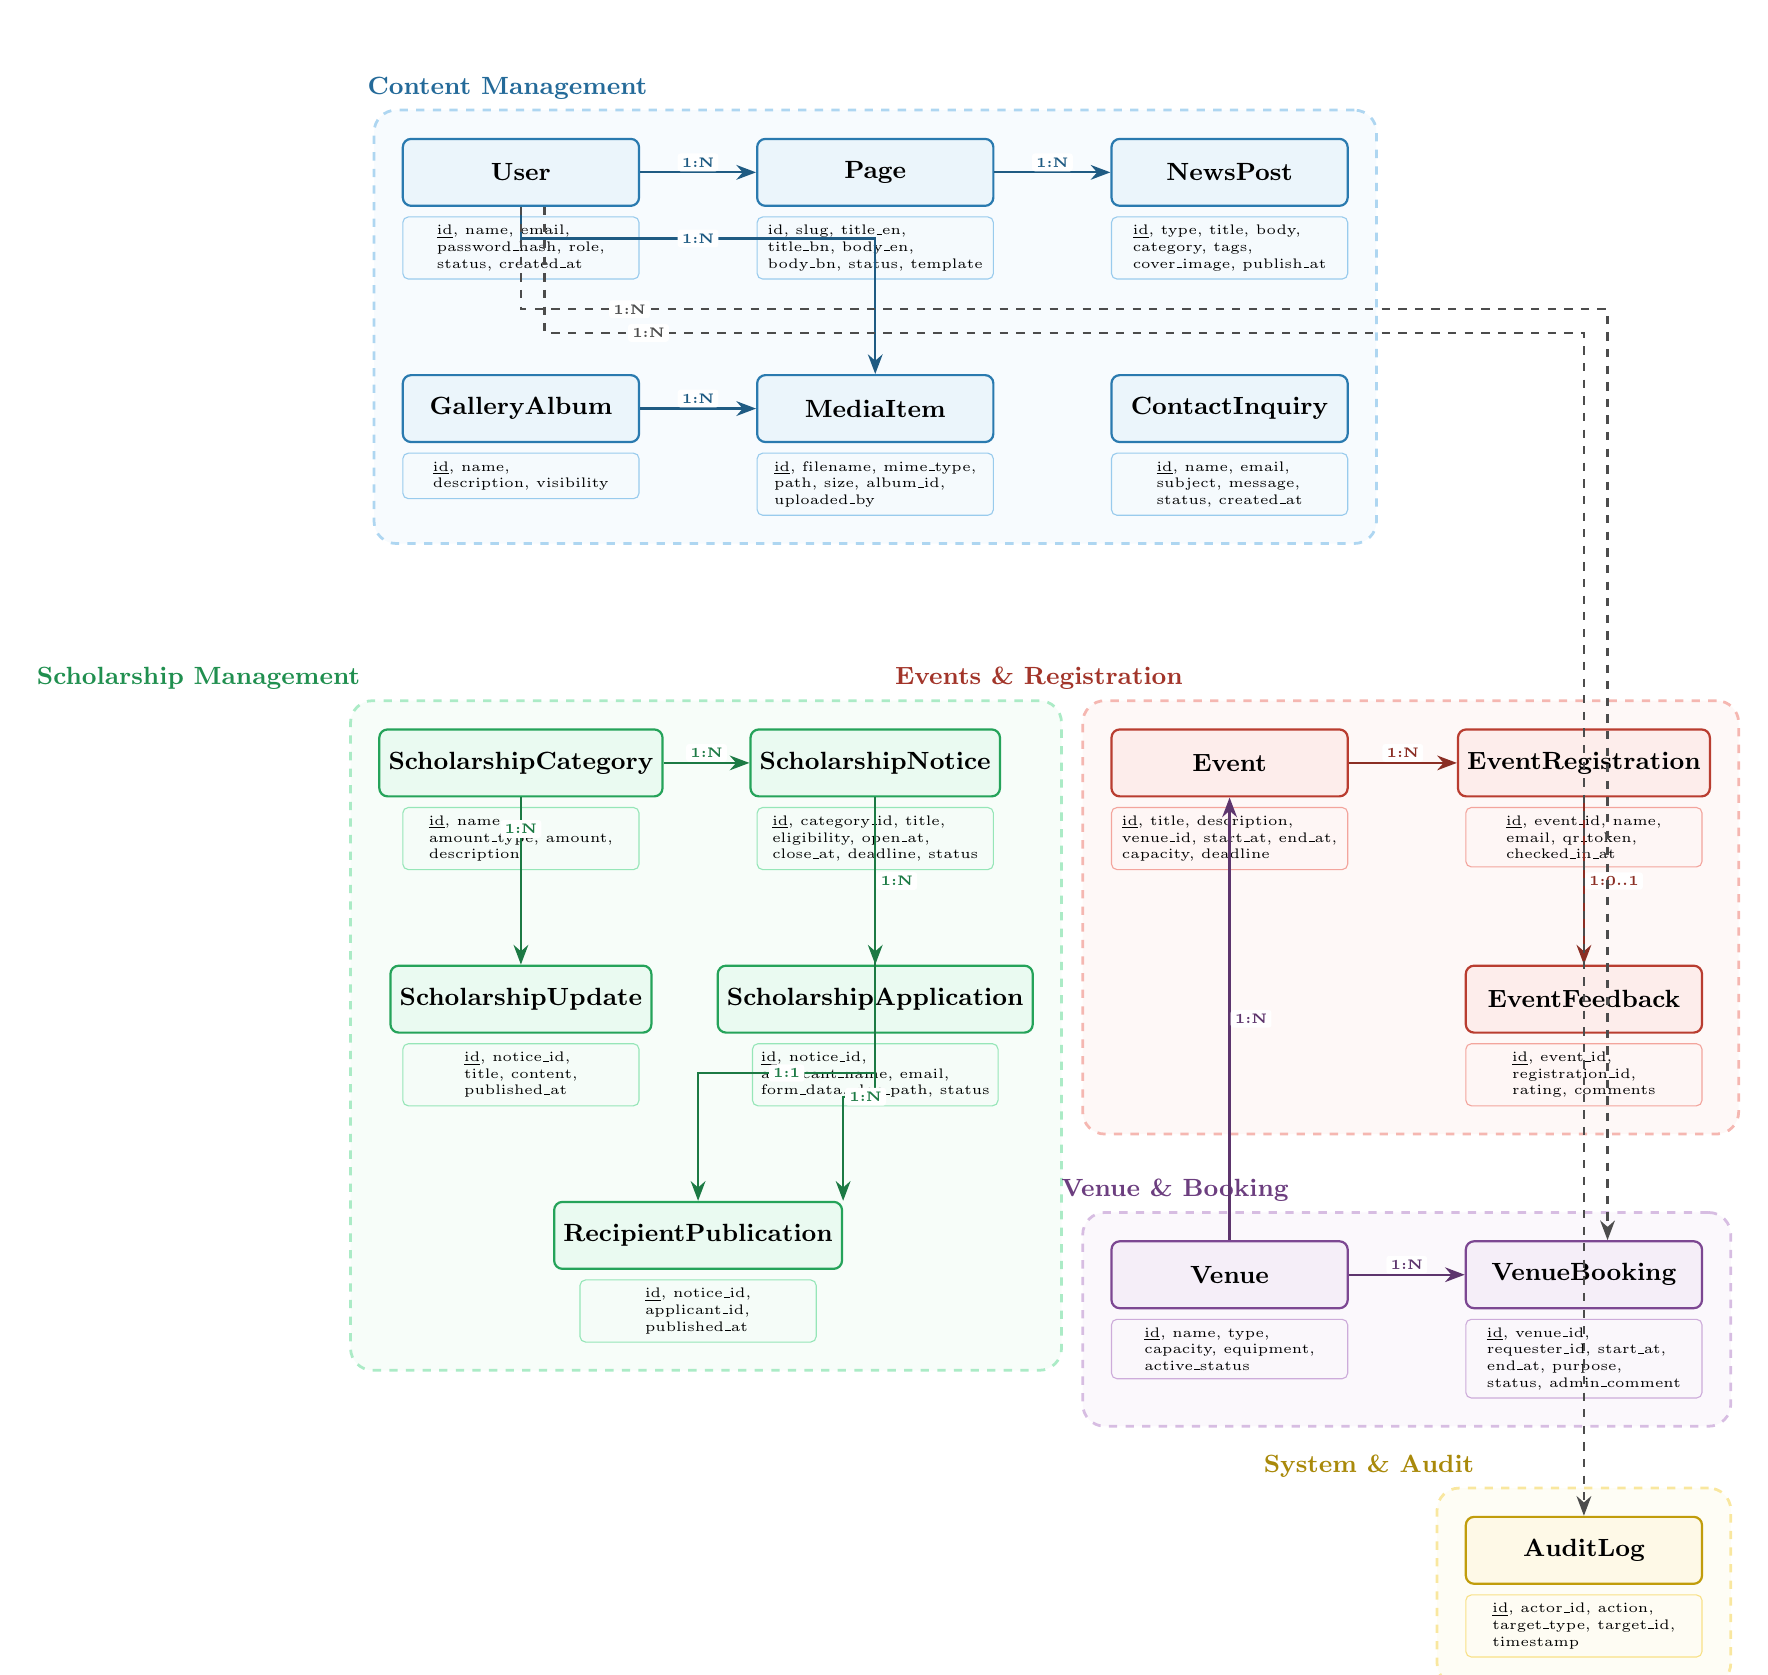
\begin{tikzpicture}[
  entity/.style={
    rectangle, draw=#1!80!black, fill=#1!10, 
    minimum width=3cm, minimum height=0.85cm, 
    font=\small\bfseries, align=center, 
    rounded corners=3pt, line width=0.8pt
  },
  attrib/.style={
    rectangle, draw=#1!50, fill=#1!5,
    minimum width=3cm, font=\tiny, align=left,
    rounded corners=2pt, inner sep=3pt
  },
  rel/.style={-{Stealth[length=2.5mm]}, thick, #1!60!black},
  relabel/.style={font=\tiny\bfseries, fill=white, inner sep=1.5pt, rounded corners=1pt},
  modbox/.style={rectangle, draw=#1!40, fill=#1!4, rounded corners=8pt, 
    inner sep=10pt, dashed, line width=1pt},
  modlabel/.style={font=\small\bfseries\color{#1!70!black}}
]

% ================================================================
% ROW 1: CONTENT MANAGEMENT MODULE (top, full width)
% ================================================================
\node[entity=modcms] (user) at (0,0) {User};
\node[attrib=modcms, below=0.12cm of user] (userattr) {
  \underline{id}, name, email,\\password\_hash, role,\\status, created\_at
};

\node[entity=modcms] (page) at (4.5,0) {Page};
\node[attrib=modcms, below=0.12cm of page] (pageattr) {
  \underline{id}, slug, title\_en,\\title\_bn, body\_en,\\body\_bn, status, template
};

\node[entity=modcms] (newspost) at (9,0) {NewsPost};
\node[attrib=modcms, below=0.12cm of newspost] (newsattr) {
  \underline{id}, type, title, body,\\category, tags,\\cover\_image, publish\_at
};

\node[entity=modcms] (album) at (0,-3) {GalleryAlbum};
\node[attrib=modcms, below=0.12cm of album] (albumattr) {
  \underline{id}, name,\\description, visibility
};

\node[entity=modcms] (media) at (4.5,-3) {MediaItem};
\node[attrib=modcms, below=0.12cm of media] (mediaattr) {
  \underline{id}, filename, mime\_type,\\path, size, album\_id,\\uploaded\_by
};

\node[entity=modcms] (inquiry) at (9,-3) {ContactInquiry};
\node[attrib=modcms, below=0.12cm of inquiry] (inqattr) {
  \underline{id}, name, email,\\subject, message,\\status, created\_at
};

% CMS module background
\begin{scope}[on background layer]
  \node[modbox=modcms, fit=(user)(userattr)(page)(pageattr)(newspost)(newsattr)(album)(albumattr)(media)(mediaattr)(inquiry)(inqattr), label={[modlabel=modcms]above left:Content Management}] {};
\end{scope}

% CMS relationships
\draw[rel=modcms] (user.east) -- node[relabel, above]{1:N} (page.west);
\draw[rel=modcms] (page.east) -- node[relabel, above]{1:N} (newspost.west);
\draw[rel=modcms] (album.east) -- node[relabel, above]{1:N} (media.west);
\draw[rel=modcms] (user.south) -- ++(0,-0.4) -| node[relabel, pos=0.25]{1:N} (media.north);

% ================================================================
% ROW 2: SCHOLARSHIP MODULE (left) + EVENTS MODULE (right)
% ================================================================

% --- Scholarship (left half) ---
\node[entity=modscholar] (schcat) at (0,-7.5) {ScholarshipCategory};
\node[attrib=modscholar, below=0.12cm of schcat] (schcatattr) {
  \underline{id}, name,\\amount\_type, amount,\\description
};

\node[entity=modscholar] (schnot) at (4.5,-7.5) {ScholarshipNotice};
\node[attrib=modscholar, below=0.12cm of schnot] (schnotattr) {
  \underline{id}, category\_id, title,\\eligibility, open\_at,\\close\_at, deadline, status
};

\node[entity=modscholar] (schapp) at (4.5,-10.5) {ScholarshipApplication};
\node[attrib=modscholar, below=0.12cm of schapp] (schappattr) {
  \underline{id}, notice\_id,\\applicant\_name, email,\\form\_data, doc\_path, status
};

\node[entity=modscholar] (schupd) at (0,-10.5) {ScholarshipUpdate};
\node[attrib=modscholar, below=0.12cm of schupd] (schupdattr) {
  \underline{id}, notice\_id,\\title, content,\\published\_at
};

\node[entity=modscholar] (recpub) at (2.25,-13.5) {RecipientPublication};
\node[attrib=modscholar, below=0.12cm of recpub] (recpubattr) {
  \underline{id}, notice\_id,\\applicant\_id,\\published\_at
};

% Scholarship module background
\begin{scope}[on background layer]
  \node[modbox=modscholar, fit=(schcat)(schcatattr)(schnot)(schnotattr)(schapp)(schappattr)(schupd)(schupdattr)(recpub)(recpubattr), label={[modlabel=modscholar]above left:Scholarship Management}] {};
\end{scope}

% Scholarship relationships
\draw[rel=modscholar] (schcat.east) -- node[relabel, above]{1:N} (schnot.west);
\draw[rel=modscholar] (schnot.south) -- node[relabel, right]{1:N} (schapp.north);
\draw[rel=modscholar] (schcat.south) -- ++(0,-0.4) -| node[relabel, pos=0.25]{1:N} (schupd.north);
\draw[rel=modscholar] (schnot.south) -- ++(0,-3.8) -| node[relabel, pos=0.15]{1:N} (recpub.north east);
\draw[rel=modscholar] (schapp.south) -- ++(0,-0.5) -| node[relabel, pos=0.25]{1:1} (recpub.north);

% --- Events (right half) ---
\node[entity=modevents] (event) at (9,-7.5) {Event};
\node[attrib=modevents, below=0.12cm of event] (eventattr) {
  \underline{id}, title, description,\\venue\_id, start\_at, end\_at,\\capacity, deadline
};

\node[entity=modevents] (eventreg) at (13.5,-7.5) {EventRegistration};
\node[attrib=modevents, below=0.12cm of eventreg] (eventregattr) {
  \underline{id}, event\_id, name,\\email, qr\_token,\\checked\_in\_at
};

\node[entity=modevents] (eventfb) at (13.5,-10.5) {EventFeedback};
\node[attrib=modevents, below=0.12cm of eventfb] (eventfbattr) {
  \underline{id}, event\_id,\\registration\_id,\\rating, comments
};

% Events module background
\begin{scope}[on background layer]
  \node[modbox=modevents, fit=(event)(eventattr)(eventreg)(eventregattr)(eventfb)(eventfbattr), label={[modlabel=modevents]above left:Events \& Registration}] {};
\end{scope}

% Event relationships
\draw[rel=modevents] (event.east) -- node[relabel, above]{1:N} (eventreg.west);
\draw[rel=modevents] (eventreg.south) -- node[relabel, right]{1:0..1} (eventfb.north);

% ================================================================
% ROW 3: VENUE MODULE (center-left) + AUDIT MODULE (right)
% ================================================================

\node[entity=modvenue] (venue) at (9,-14) {Venue};
\node[attrib=modvenue, below=0.12cm of venue] (venueattr) {
  \underline{id}, name, type,\\capacity, equipment,\\active\_status
};

\node[entity=modvenue] (booking) at (13.5,-14) {VenueBooking};
\node[attrib=modvenue, below=0.12cm of booking] (bookingattr) {
  \underline{id}, venue\_id,\\requester\_id, start\_at,\\end\_at, purpose,\\status, admin\_comment
};

% Venue module background
\begin{scope}[on background layer]
  \node[modbox=modvenue, fit=(venue)(venueattr)(booking)(bookingattr), label={[modlabel=modvenue]above left:Venue \& Booking}] {};
\end{scope}

% Venue relationships
\draw[rel=modvenue] (venue.east) -- node[relabel, above]{1:N} (booking.west);
\draw[rel=modvenue] (venue.north) -- node[relabel, right]{1:N} (event.south);

% --- Audit ---
\node[entity=modsystem] (audit) at (13.5,-17.5) {AuditLog};
\node[attrib=modsystem, below=0.12cm of audit] (auditattr) {
  \underline{id}, actor\_id, action,\\target\_type, target\_id,\\timestamp
};

% Audit module background
\begin{scope}[on background layer]
  \node[modbox=modsystem, fit=(audit)(auditattr), label={[modlabel=modsystem]above left:System \& Audit}] {};
\end{scope}

% ================================================================
% CROSS-MODULE RELATIONSHIPS (dashed gray)
% ================================================================
\draw[rel=gray, dashed] (user.south) -- ++(0,-1.3) -| node[relabel, pos=0.05]{1:N} ([xshift=0.3cm]booking.north);
\draw[rel=gray, dashed] ([xshift=0.3cm]user.south) -- ++(0,-1.6) -| node[relabel, pos=0.05]{1:N} (audit.north);

\end{tikzpicture}
}%
\caption{Entity-Relationship Diagram -- Project A: Department Website, CMS, Scholarship, Events, and Venue Booking System}
\label{fig:erdiagram}
\end{figure}

% \section{Appendix B: Suggested Wireframes}

% The final report should attach wireframes for the public homepage, CMS page editor, scholarship application form, scholarship dashboard, event listing/registration page, QR check-in interface, and venue booking calendar.

\end{document}